\documentclass[tikz,border=6pt]{standalone}
\usepackage{amsmath}
\usepackage{xcolor}
\usetikzlibrary{arrows.meta,positioning,calc,fit}

% Reproducible paper-style source for assets/diagrams/dynur.svg
% Build:
%   pdflatex -interaction=nonstopmode -halt-on-error dynur.tex
%   dvisvgm --pdf --no-fonts --exact-bbox dynur.pdf -o ../dynur.svg

\definecolor{ink}{HTML}{203746}
\definecolor{muted}{HTML}{647783}
\definecolor{line}{HTML}{AFC2CE}
\definecolor{panel}{HTML}{F8FAFB}
\definecolor{blue1}{HTML}{E6F0F5}
\definecolor{blue2}{HTML}{C9DDE8}
\definecolor{blue3}{HTML}{92B9CD}
\definecolor{blue4}{HTML}{4D86A4}
\definecolor{orange}{HTML}{D77A3B}
\definecolor{orangefill}{HTML}{F6E5D8}

\tikzset{
  >={Stealth[length=2.4mm,width=1.7mm]},
  flow/.style={->, draw=muted, line width=0.9pt},
  panelbox/.style={draw=line, fill=panel, rounded corners=2.2mm, line width=0.65pt},
  smalllabel/.style={font=\scriptsize, text=muted},
  panellabel/.style={font=\bfseries\small, text=ink},
  body/.style={font=\small, text=ink},
  tinybody/.style={font=\scriptsize, text=ink},
}

\begin{document}
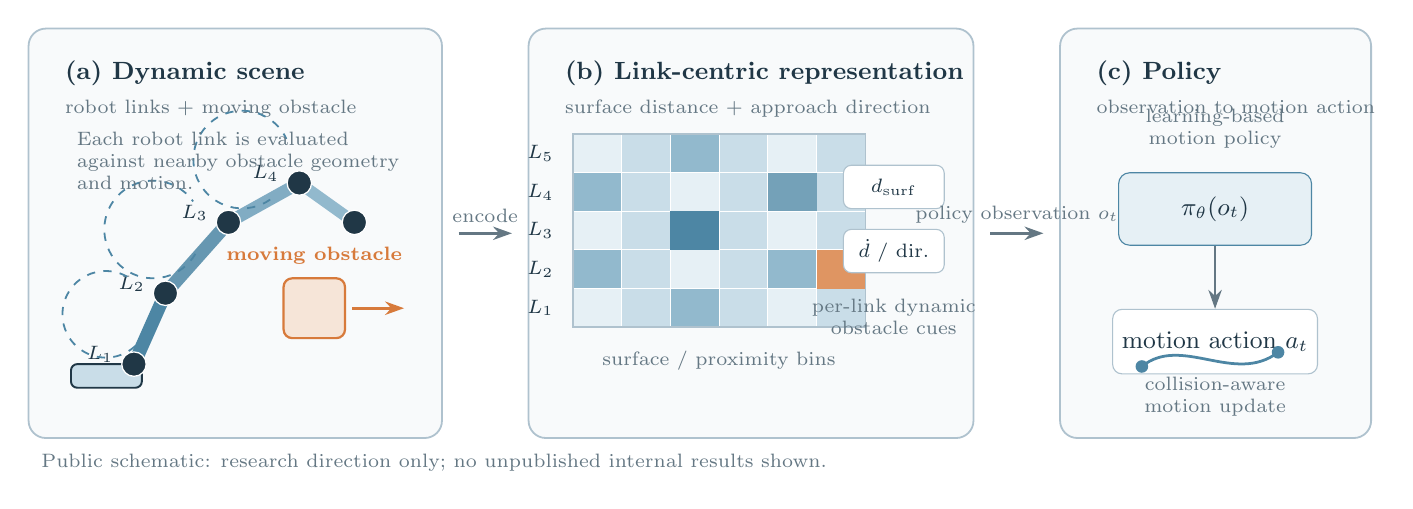
\begin{tikzpicture}[x=1cm,y=1cm, font=\sffamily]

% -----------------------------------------------------------------------------
% Panel A: dynamic robot scene
% -----------------------------------------------------------------------------
\node[panelbox, minimum width=5.25cm, minimum height=5.2cm, anchor=south west] (scene) at (0,0) {};
\node[panellabel, anchor=north west] at ([xshift=3.5mm,yshift=-3mm]scene.north west) {(a) Dynamic scene};
\node[smalllabel, anchor=north west] at ([xshift=3.5mm,yshift=-8mm]scene.north west) {robot links + moving obstacle};

% base
\filldraw[draw=ink, fill=blue2, line width=0.7pt, rounded corners=0.8mm]
  (0.55,0.65) rectangle (1.45,0.95);

% arm geometry
\coordinate (j0) at (1.35,0.95);
\coordinate (j1) at (1.75,1.85);
\coordinate (j2) at (2.55,2.75);
\coordinate (j3) at (3.45,3.25);
\coordinate (j4) at (4.15,2.75);
\draw[line width=4.8pt, draw=blue4, line cap=round] (j0)--(j1);
\draw[line width=4.8pt, draw=blue4!86!white, line cap=round] (j1)--(j2);
\draw[line width=4.5pt, draw=blue3!75!blue4, line cap=round] (j2)--(j3);
\draw[line width=4.2pt, draw=blue3, line cap=round] (j3)--(j4);
\foreach \p in {j0,j1,j2,j3,j4}{\filldraw[fill=ink,draw=white,line width=0.45pt] (\p) circle (1.55mm);}

% link labels and local proximity arcs
\node[tinybody, anchor=east] at ($(j0)+(-0.14,0.12)$) {$L_1$};
\node[tinybody, anchor=east] at ($(j1)+(-0.14,0.12)$) {$L_2$};
\node[tinybody, anchor=east] at ($(j2)+(-0.14,0.12)$) {$L_3$};
\node[tinybody, anchor=east] at ($(j3)+(-0.14,0.12)$) {$L_4$};
\draw[dashed, draw=blue4, line width=0.65pt] (1.49,1.35) arc[start angle=335,end angle=55,radius=0.55];
\draw[dashed, draw=blue4, line width=0.65pt] (2.13,2.35) arc[start angle=330,end angle=35,radius=0.62];
\draw[dashed, draw=blue4, line width=0.65pt] (3.08,3.04) arc[start angle=305,end angle=25,radius=0.62];

% moving obstacle
\filldraw[fill=orangefill, draw=orange, line width=0.8pt, rounded corners=1.1mm]
  (3.25,1.28) rectangle (4.03,2.04);
\draw[->, draw=orange, line width=0.95pt] (4.12,1.66) -- (4.78,1.66);
\node[font=\scriptsize\bfseries, text=orange, anchor=south] at (3.64,2.10) {moving obstacle};
\node[smalllabel, anchor=north west, text width=4.35cm] at (0.5,4.02) {Each robot link is evaluated against nearby obstacle geometry and motion.};

% -----------------------------------------------------------------------------
% Panel B: link-centric observation
% -----------------------------------------------------------------------------
\node[panelbox, minimum width=5.65cm, minimum height=5.2cm, anchor=south west] (repr) at (6.35,0) {};
\node[panellabel, anchor=north west] at ([xshift=3.5mm,yshift=-3mm]repr.north west) {(b) Link-centric representation};
\node[smalllabel, anchor=north west] at ([xshift=3.5mm,yshift=-8mm]repr.north west) {surface distance + approach direction};

% matrix/grid
\coordinate (g0) at (6.92,1.42);
\def\cw{0.62}
\def\ch{0.49}
\foreach \r in {0,...,4}{
  \foreach \c in {0,...,5}{
    \pgfmathtruncatemacro{\tone}{mod(2*\r+\c,4)}
    \ifcase\tone\def\cellcolor{blue1}\or\def\cellcolor{blue2}\or\def\cellcolor{blue3}\or\def\cellcolor{blue2}\fi
    \filldraw[fill=\cellcolor, draw=white, line width=0.35pt]
      ($(g0)+(\c*\cw,\r*\ch)$) rectangle ++(\cw,\ch);
  }
}
\draw[draw=line, line width=0.7pt] (g0) rectangle ++(3.72,2.45);

% emphasized cells
\fill[blue4] ($(g0)+(1.24,0.98)$) rectangle ++(0.62,0.49);
\fill[blue4!78!white] ($(g0)+(2.48,1.47)$) rectangle ++(0.62,0.49);
\fill[orange!80!white] ($(g0)+(3.10,0.49)$) rectangle ++(0.62,0.49);

\foreach \r/\lab in {0/$L_1$,1/$L_2$,2/$L_3$,3/$L_4$,4/$L_5$}{
  \node[tinybody, anchor=east] at ($(g0)+(-0.12,\r*\ch+0.245)$) {\lab};
}
\node[smalllabel, anchor=north] at ($(g0)+(1.86,-0.18)$) {surface / proximity bins};

% side features
\node[draw=line, fill=white, rounded corners=1mm, minimum width=1.28cm, minimum height=0.55cm,
      font=\scriptsize, text=ink] (dist) at (11.00,3.20) {$d_{\mathrm{surf}}$};
\node[draw=line, fill=white, rounded corners=1mm, minimum width=1.28cm, minimum height=0.55cm,
      font=\scriptsize, text=ink, below=2.5mm of dist] (approach) {$\dot d$ / dir.};
\node[smalllabel, align=center, below=2mm of approach] {per-link dynamic\\obstacle cues};

% flow from scene to repr
\draw[flow] ([xshift=2mm]scene.east) -- node[above, font=\scriptsize, text=muted] {encode} ([xshift=-2mm]repr.west);

% -----------------------------------------------------------------------------
% Panel C: policy/action
% -----------------------------------------------------------------------------
\node[panelbox, minimum width=3.95cm, minimum height=5.2cm, anchor=south west] (policy) at (13.10,0) {};
\node[panellabel, anchor=north west] at ([xshift=3.5mm,yshift=-3mm]policy.north west) {(c) Policy};
\node[smalllabel, anchor=north west] at ([xshift=3.5mm,yshift=-8mm]policy.north west) {observation to motion action};

\node[draw=blue4, fill=blue1, rounded corners=1.4mm, minimum width=2.45cm, minimum height=0.92cm,
      font=\small\bfseries, text=ink] (pi) at (15.08,2.92) {$\pi_{\theta}(o_t)$};
\node[smalllabel, align=center, above=1.8mm of pi] {learning-based\\motion policy};

\node[draw=line, fill=white, rounded corners=1.2mm, minimum width=2.55cm, minimum height=0.82cm,
      font=\small, text=ink, below=8mm of pi] (action) {motion action $a_t$};
\draw[flow] (pi) -- (action);

% small trajectory icon
\draw[draw=blue4, line width=1.0pt] (14.15,0.92) .. controls (14.65,1.33) and (15.33,0.68) .. (15.88,1.10);
\fill[blue4] (14.15,0.92) circle (0.8mm);
\fill[blue4] (15.88,1.10) circle (0.8mm);
\node[smalllabel, align=center] at (15.08,0.54) {collision-aware\\motion update};

\draw[flow] ([xshift=2mm]repr.east) -- node[above, font=\scriptsize, text=muted] {policy observation $o_t$} ([xshift=-2mm]policy.west);

% global bottom note
\node[font=\scriptsize, text=muted, anchor=west] at (0.05,-0.30)
  {Public schematic: research direction only; no unpublished internal results shown.};

\end{tikzpicture}
\end{document}
